% !TeX spellcheck = en_US
% !TeX root = tikz-ext-manual.tex
% Copyright 2022 by Qrrbrbirlbel
%
% This file may be distributed and/or modified
%
% 1. under the LaTeX Project Public License and/or
% 2. under the GNU Free Documentation License.
%
\newcommand*\tikzextname{Ti\emph{k}Z-Extensions}
\newcommand*\tikzextversion{0.1}
\begin{document}

\title{\bfseries The \tikzextname\space Package\\
  \large Manual for version \tikzextversion\\[1mm]
%\large\href{https://github.com/pgf-tikz/pgf}{\texttt{https://github.com/pgf-tikz/pgf}}}
\author{Qrrbrbirlbel}}

\maketitle
\label{table-of-contents}

\tableofcontents

\clearpage
\part{Introduction}
\begin{multicols}{2}
\section{Usage}
This package is called |tikz-ext|, however, one can't load it via |\usepackage|.
Instead, this package consists of multiple PGF and \tikzname\space libraries
which are loaded by either |\usepgflibrary| or |\usetikzlibrary|.

\section{Why do we need it?}
Since I have been answering questions on \hyperlink{https://tex.stackexchange.com}{TeX.sx}
I've noticed that some questions come up again and again,
every time with a slightly different approach on how to solve them.

I don't like reinventing the wheel which is why I've gathered the code of my answers in this package.

And, yes, I am using them myself, too.

\section{Should these libraries be part of \tikzname?}
I guess.
\end{multicols}

\clearpage
\part{\tikzname\space Libraries}

% !TeX root = tikz-ext-manual.tex
% !TeX spellcheck = en_US
% Copyright 2022 by Qrrbrbirlbel
%
% This file may be distributed and/or modified
%
% 1. under the LaTeX Project Public License and/or
% 2. under the GNU Free Documentation License.
%

\section{More Horizontal and Vertical Lines}
\label{library:paths.ortho}

\begin{tikzlibrary}{ext.paths.ortho}
  This library adds new path specifications \verb!|-|!, \verb!-|-! as well as
  |r-ud|, |r-du|, |r-lr| and |r-rl|.
\end{tikzlibrary}

\subsection{Zig-Zag}
Similar to the path operations \verb!|-! and \verb!-|! this library adds\indexPathOperationO{\protect\pgfmanualbar-}\indexPathOperationO{-\protect\pgfmanualbar}
the path operations \verb!|-|! and \verb!-|-!.
{\catcode`\|=12
\begin{pathoperation}[noindex]{|-|}{\opt{\oarg{options}}\meta{coordinate or cycle}}
    \index{---1@\protect\texttt{\protect\pgfmanualbar-\protect\pgfmanualbar} path operation}%
    \index{Path operations!---1@\protect\texttt{\protect\pgfmanualbar-\protect\pgfmanualbar}}%
    \pgfmanualpdflabel[\catcode`\|=12 ]{|-|}{}%
    This operation means ``first vertical, then horizontal and then vertical again''.
\end{pathoperation}
\begin{pathoperation}[noindex]{-|-}{\opt{\oarg{options}}\meta{coordinate or cycle}}
    \index{--1@\protect\texttt{-\protect\pgfmanualbar-} path operation}%
    \index{Path operations!--1@\protect\texttt{-\protect\pgfmanualbar-}}%
    \pgfmanualpdflabel[\catcode`\|=12 ]{-|-}{}%
    This operation means ``first horizontal, then vertical and then horizontal again''.
\end{pathoperation}
}
\begin{key}{/tikz/ortho/ratio=\meta{ratio} (initially 0.5)}
  This sets the ratio for the middle part of the Zig-Zag connection.
  
  For values $\meta{ratio} < 0$ and $\meta{ratio} > 1$ the Zig-Zag lines will
  look more like Zig-Zig lines.
\begin{codeexample}[preamble=\usetikzlibrary{paths.ortho}]
\begin{tikzpicture}[very thick, rounded corners]
\draw[help lines] (-.25, -1.25) grid (2.25, 1.25);
\draw (0, 0) -|-            (2, 1) --
      (2, 0) -|-[ratio=.25] (0,-1) -- cycle;
\end{tikzpicture}
\end{codeexample}
\end{key}
%TODO: hvvh/distance needs fixing, maybe?
\begin{key}{/tikz/ortho/distance=\meta{distance}}
  This sets the distance between the start point
  and the middle part of the Zig-Zag connection.
  
  For values $\meta{distance} < 0$ the distance will be used for the target coordinate.
\begin{codeexample}[width=8cm,preamble=\usetikzlibrary{ext.paths.ortho}]
\begin{tikzpicture}[very thick,-latex]
\draw[help lines,-] (-.25, -.25) grid (5.25, 3.25);
\draw (0, 0) -|-[distance= .5cm] ++(2, 1);
\draw (0, 2) -|-[distance=-.5cm] ++(2, 1);

\tikzset{xshift=3cm}
\draw (2, 1) -|-[distance= .5cm] ++(-2, -1);
\draw (2, 3) -|-[distance=-.5cm] ++(-2, -1);
\end{tikzpicture}
\end{codeexample}
\end{key}
\begin{key}{/tikz/ortho/from center=\opt{\meta{true or false}} (default true)}
  When nodes get connected the placement of the middle part of the Zig-Zag
  and the Zig-Zig (see below) connections will be calculated from the border
  of these nodes.
  The middle part of the connections can be calculated from the nodes' center
  if this key is set to |true|.
\end{key}

New timers are setup for both the Zig-Zag and the Zig-Zig connections,
these can be configured through the following keys.
\begin{codeexample}[width=8cm,preamble=\usetikzlibrary{paths.ortho}]
\tikz \draw (0,0) -|- (2,3) 
  foreach \p in {0.0, 0.25, 0.5, 0.75, 1.0}{
    node [pos=\p] {\p}};
\end{codeexample}
\begin{key}{/tikz/ortho/spacing=\meta{number} (initially 4)}
  Unless $\meta{number} = 0$ is set
  \begin{itemize}
  \item |pos = 0| will be at the start,\indexKeyO{pos}
  \item |pos = 1| will be at the end,
  \item |pos = |$\frac{1}{\meta{number}}$ will be at the first kink,
  \item |pos = |$\frac{\meta{number}-1}{\meta{number}}$ will be at the second kink and
  \item |pos = .5| will be in the middle of the middle part of the connection.
  \end{itemize}
  
  If $\meta{number} = 0$ then
  \begin{itemize}
  \item |pos = -1| will be at the start,
  \item |pos = 2| will be at the end,
  \item |pos = 0| will be at the first kink,
  \item |pos = 1| will be at the second kink and
  \item |pos = .5| will still be in the middle of the middle part of the connection.
  \end{itemize}
\end{key}
\begin{key}{/tikz/ortho/middle 0 to 1}
  This is an alias for |spacing = 0|.
\end{key}

\subsection{Zig-Zig}
\begin{pathoperation}{r-ud}{\opt{\oarg{options}}\meta{coordinate or cycle}}
  This operation means ``first up, then horizontal and then down''.
  \begin{key}{/tikz/ortho/ud distance=\meta{length} (initially .5cm)}
    This sets the distance between the start and the horizontal line to \meta{length}.
  \end{key}
\end{pathoperation}
\begin{pathoperation}{r-du}{\opt{\oarg{options}}\meta{coordinate or cycle}}
  This operation means ``first down, then horizontal and then up''.
  \begin{key}{/tikz/ortho/du distance=\meta{length} (initially .5cm)}
    This sets the distance between the start and the horizontal line to \meta{length}.
  \end{key}
\end{pathoperation}
\begin{pathoperation}{r-lr}{\opt{\oarg{options}}\meta{coordinate or cycle}}
  This operation means ``left down, then vertical and then right''.
  \begin{key}{/tikz/ortho/lr distance=\meta{length} (initially .5cm)}
    This sets the distance between the start and the vertical line to \meta{length}.
  \end{key}
\end{pathoperation}
\begin{pathoperation}{r-rl}{\opt{\oarg{options}}\meta{coordinate or cycle}}
  This operation means ``first right, then vertical and then down''.
  \begin{key}{/tikz/ortho/rl distance=\meta{length} (initially .5cm)}
    This sets the distance between the start and the vertical line to \meta{length}.
  \end{key}
\end{pathoperation}

All distances can be set with one key.
\begin{key}{/tikz/ortho/udlr distance=\meta{length}}
  Sets all the previous distances to the same value \meta{length}.
\end{key}

\subsection{Even more Horizontal and Vertical Lines}

The following keys can be used to access vertical and horizontal line path operations.
\begin{stylekey}{/tikz/horizontal vertical}
  This installs  \verb!to path = -| (\tikztotarget) \tikztonodes!\indexKeyO{to path}
  that can be used with the path operations |to| or |edge|.
\end{stylekey}
\begin{stylekey}{/tikz/vertical horizontal}
  This installs \verb!to path = |- (\tikztotarget) \tikztonodes!
  that can be used with the path operations |to| or |edge|.
\end{stylekey}
\begin{stylekey}{/tikz/horizontal vertical horizontal}
  This installs  \verb!to path = -|- (\tikztotarget) \tikztonodes!
  that can be used with the path operations |to| or |edge|.
\end{stylekey}
\begin{stylekey}{/tikz/vertical horizontal vertical}
  This installs  \verb!to path = |-| (\tikztotarget) \tikztonodes!
  that can be used with the path operations |to| or |edge|.
\end{stylekey}

When connecting rectangular nodes, these keys could be useful as well.
They all need to be given to a |to| or |edge| path operation.
\begin{stylekey}{/tikz/only vertical second=\opt{\meta{length}} (default 0pt)}
This draws a vertical line from the start point to the target point so that
it connects to the target point in the center (or at its border in case it is a node).

The optional \meta{length} can be used to shift the line orthogonally to its direction.
\end{stylekey}
\begin{stylekey}{/tikz/only horizontal second=\opt{\meta{length}} (default 0pt)}
This draws a horizontal line from the start point to the target point so that
it connects to the target point in the center (or at its border in case it is a node).

The optional \meta{length} can be used to shift the line orthogonally to its direction.
\end{stylekey}
\begin{stylekey}{/tikz/only vertical first=\opt{\meta{length}} (default 0pt)}
This draws a vertical line from the start point to the target point so that
it connects to the start point in the center (or at its border in case it is a node).

The optional \meta{length} can be used to shift the line orthogonally to its direction.
\end{stylekey}
\begin{stylekey}{/tikz/only horizontal first=\opt{\meta{length}} (default 0pt)}
This draws a horizontal line from the start point to the target point so that
it connects to the start point in the center (or at its border in case it is a node).

The optional \meta{length} can be used to shift the line orthogonally to its direction.
\end{stylekey}

\pagebreak
Since all previous key are rather cumbersome, one can install shortcuts for these.
\begin{stylekey}{/tikz/ortho/install shortcuts}
Installs the following shortcuts:\\
{\ttfamily
\begin{tabular}{l@{\hspace{.5em}${}\to{}$\hspace{.5em}}l}
  \pgfmanualbar-              & vertical horizontal            \\
  -\pgfmanualbar              & horizontal vertical            \\
  -\pgfmanualbar-             & horizontal vertical horizontal \\
  \pgfmanualbar-\pgfmanualbar & vertical horizontal vertical   \\
  \pgfmanualbar*              & only vertical first            \\
  *\pgfmanualbar              & only vertical second           \\
  -*                          & only horizontal first          \\
  *-                          & only horizontal second
\end{tabular}
}
\end{stylekey}

% !TeX root = tikz-ext-manual.tex
% !TeX spellcheck = en_US
% Copyright 2022 by Qrrbrbirlbel
%
% This file may be distributed and/or modified
%
% 1. under the LaTeX Project Public License and/or
% 2. under the GNU Free Documentation License.
%

\section{Extending the Path Timers}
\label{library:timer}

\begin{tikzlibrary}{paths.timer}
  This library adds timers to the path specifications |rectangle|, |parabola|, |sin| and |cos|.
\end{tikzlibrary}

In \tikzname, the path specification |rectangle|, |parabola|, |sin| and |cos| do not provide
their own timer, i.\,e. a node placing algorithm that is dependent on the actual path.
For |rectangle| the timer of the straight line between the rectangle's corners is used, for
the other paths, nodes, coordinates, pics, etc. are placed on the last coordinate.

This library allows this.

\subsection{Rectangle}
For the |rectangle| path operator, the timer starts with |pos = 0| (= |at start|) from
the starting coordinate in a counter-clockwise direction along the rectangle.
The corners will be at positions 0.0, 0.25, 0.5, 0.75 and 1.0.

\begin{codeexample}[width=10cm,preamble=\usetikzlibrary{paths.timer}]
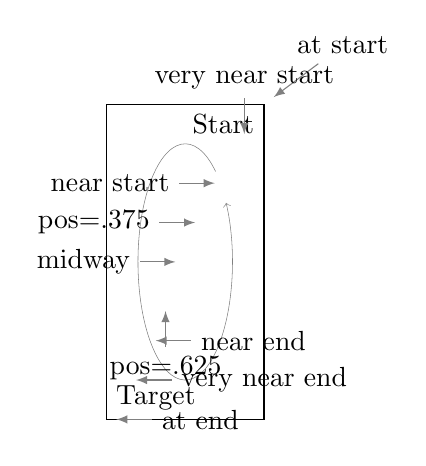
\begin{tikzpicture}[scale=2, every pin edge/.style={latex-, gray}]
\coordinate [label=above right:Target] (A) at (0,0);
\coordinate [label=below left:Start]   (B) at (1,2);
\draw[->, help lines] ([shift=(50:.3 and .75)] .5,1)
  arc[start angle=50, delta angle=340, x radius=.3, y radius=.75];
\draw (B) rectangle (A)
  foreach \pos/\ang in {at start/60, very near start/90, near start/180, pos=.375/180,
                        midway/180, pos=.625/270, near end/0, very near end/0, at end/0}{
    node[pin=\ang:\pos, style/.expanded=\pos]{}};
\end{tikzpicture}
\end{codeexample}

\subsection{Parabola}

For the |parabola| path operator the timer is similar to the |.. controls ..| operator.

The position 0.5 will lie at the |bend|.
\begin{codeexample}[width=.3\linewidth,preamble=\usetikzlibrary{paths.timer}]
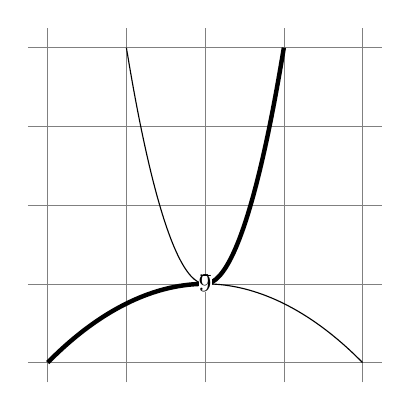
\begin{tikzpicture}
\draw[help lines]  (-2.25, -1.25) grid (2.25, 3.25);
\draw              ( 2,-1) parabola bend (0,0) (-1,3);
\draw[ultra thick] (-2,-1) parabola bend (0,0) ( 1,3)
  foreach \pos in {1,...,4,6,7,...,9}{
    node[
      pos=.\pos, sloped, fill=white, font=\small, inner sep=+0pt
    ] {\pos}
  };
\end{tikzpicture}
\end{codeexample}

If no |bend| is specified half the positions will collapse into one end of the curve.

\begin{codeexample}[width=.3\linewidth,preamble=\usetikzlibrary{paths.timer}]
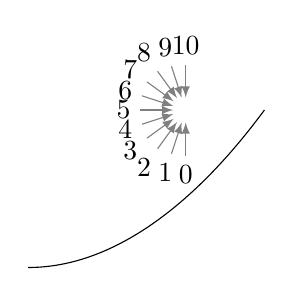
\begin{tikzpicture}[every pin edge/.style={latex-, shorten <=1pt, gray}]
\draw (-2,-2) parabola (1,0)
  foreach \pos in {0, 1, ..., 10} {
    node [pos=\pos/10, pin={[anchor=-18*\pos+90]-18*\pos+270:\pos}]{}
  };
\end{tikzpicture}
\end{codeexample}

\subsection{Sine/Cosine}

The |sin| and |cos| path operators also allow placing of nodes along their paths.

\begin{codeexample}[width=.3\linewidth,preamble=\usetikzlibrary{paths.timer}]
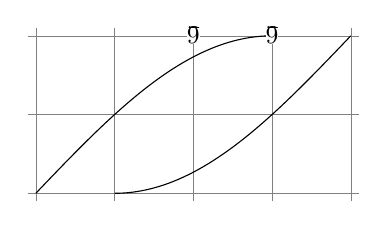
\begin{tikzpicture}[mark nodes on line/.style={insert path={
  foreach \pos in {1, ..., 9} {node[
    sloped, fill=white, font=\small, inner sep=+0pt, pos=\pos/10] {\pos}}}}]
\draw[help lines] (-2.1,-2.1) grid (2.1,0.1);
\draw             (-2,-2) sin (1,0) [mark nodes on line];
\draw[shift=(0:1)](-2,-2) cos (1,0) [mark nodes on line];
\end{tikzpicture}
\end{codeexample}

\endinput
% Copyright 2022 by Qrrbrbirlbel
%
% This file may be distributed and/or modified
%
% 1. under the LaTeX Project Public License and/or
% 2. under the GNU Free Documentation License.
%

\clearpage
\section{Mirror, Mirror on the Wall}
\label{library:mirror}

\begin{tikzlibrary}{ext.transformations.mirror}
  This library adds more transformations to \tikzname.
\end{tikzlibrary}

As explained in section~\ref{pgflibrary:transformations}, they are two approaches to setting a mirror transformation.
As with the commands in PGF, we'll be using lowercase |m| for the ``Spiegelungsmatrix'' and uppercase |M| for the built-in approach.

\subsection{Using the ``Spiegelungsmatrix''}

\begin{codeexample}[width=.4\linewidth,preamble=\usetikzlibrary{shapes.geometric,ext.transformations.mirror}]
\begin{tikzpicture}[line join=round, thick, reg poly/.style={
  shape=regular polygon, regular polygon sides={#1}}]
\node[reg poly=5, minimum size=+2cm, draw, very thick] (a) {};
\foreach \i[evaluate={\col=(\i-1)/.04}] in {1,...,5}
  \node [mirror=(a.corner \i)--(a.side \i), transform shape,
         reg poly=5, minimum size=+2cm, draw=red!\col!blue] {};
\end{tikzpicture}
\end{codeexample}

\begin{key}{/tikz/xmirror=\meta{value or coordinate}}
  Sets up a transformation that mirrors along a horizontal line that goes through point $(\text{\meta{value}}, 0)$ or \meta{coordinate}.

\begin{codeexample}[preamble=\usetikzlibrary{ext.transformations.mirror}]
\begin{tikzpicture}
\draw[help lines] (-0.25, -.25) grid (3.25, 1.25);
\draw[-latex] (0,0) .. controls (.5,1) .. (1,1);

\draw[dashed] (1.5, -.25) coordinate (m) -- (1.5, 1.25);
\draw[xmirror=(m),-latex] (0,0) .. controls (.5,1) .. (1,1);
\end{tikzpicture}
\end{codeexample}
\end{key}

\begin{key}{/tikz/ymirror=\meta{value or coordinate}}
  Sets up a transformation that mirrors along a vertical line that goes through point $(0, \text{\meta{value}})$ or \meta{coordinate}.
\end{key}


\begin{key}{/tikz/mirror x=\meta{coordinate}}
  Similar to |/tikz/xmirror|, this however uses the |xyz| coordinate system instead of the |canvas| system.
\begin{codeexample}[preamble=\usetikzlibrary{ext.transformations.mirror}]
\begin{tikzpicture}[x=.5cm, y=(45:1cm)]

\draw[-latex] (0,0) .. controls (.5,1) .. (1,1);

\draw[dashed] (1.5, -.25) coordinate (m) -- (1.5, 1.25);

\draw[ xmirror=(m), -latex, red, dotted] (0,0) .. controls (.5,1) .. (1,1);
\draw[mirror x=(m), -latex]              (0,0) .. controls (.5,1) .. (1,1);
\end{tikzpicture}
\end{codeexample}
\end{key}

\begin{key}{/tikz/mirror y=\meta{coordinate}}
  Similar to |/tikz/ymirror|, this however uses the |xyz| coordinate system instead of the |canvas| system.
\end{key}


\begin{key}{/tikz/mirror=\meta{point A}|--|\meta{point B}}
  Sets up a transformation that mirrors along a line that goes through \meta{point A} and \meta{point B}.
  
  When only \meta{point A} is given that line goes through \meta{point A} and the origin.
\end{key}

\subsection{Using built-in transformations}

\begin{codeexample}[width=.4\linewidth,preamble=\usetikzlibrary{shapes.geometric,ext.transformations.mirror}]
\begin{tikzpicture}[line join=round, thick, reg poly/.style={
  shape=regular polygon, regular polygon sides={#1}}]
\node[reg poly=5, minimum size=+2cm, draw, very thick] (a) {};
\foreach \i[evaluate={\col=(\i-1)/.04}] in {1,...,5}
  \node [Mirror=(a.corner \i)--(a.side \i), transform shape,
         reg poly=5, minimum size=+2cm, draw=red!\col!blue] {};
\end{tikzpicture}
\end{codeexample}

\begin{key}{/tikz/xMirror=\meta{value or coordinate}}
  Sets up a transformation that mirrors along a horizontal line that goes through point $(\text{\meta{value}}, 0)$ or \meta{coordinate}.

\begin{codeexample}[preamble=\usetikzlibrary{ext.transformations.mirror}]
\begin{tikzpicture}
\draw[help lines] (-0.25, -.25) grid (3.25, 1.25);
\draw[-latex] (0,0) .. controls (.5,1) .. (1,1);

\draw[dashed] (1.5, -.25) coordinate (m) -- (1.5, 1.25);
\draw[xMirror=(m),-latex] (0,0) .. controls (.5,1) .. (1,1);
\end{tikzpicture}
\end{codeexample}
\end{key}

\begin{key}{/tikz/yMirror=\meta{value or coordinate}}
  Sets up a transformation that mirrors along a vertical line that goes through point $(0, \text{\meta{value}})$ or \meta{coordinate}.
\end{key}


\begin{key}{/tikz/Mirror x=\meta{coordinate}}
  Similar to |/tikz/xMirror|, this however uses the |xyz| coordinate system instead of the |canvas| system.
\begin{codeexample}[preamble=\usetikzlibrary{ext.transformations.mirror}]
\begin{tikzpicture}[x=.5cm, y=(45:1cm)]

\draw[-latex] (0,0) .. controls (.5,1) .. (1,1);

\draw[dashed] (1.5, -.25) coordinate (m) -- (1.5, 1.25);

\draw[ xMirror=(m), -latex, red, dotted] (0,0) .. controls (.5,1) .. (1,1);
\draw[Mirror x=(m), -latex]              (0,0) .. controls (.5,1) .. (1,1);
\end{tikzpicture}
\end{codeexample}
\end{key}

\begin{key}{/tikz/Mirror y=\meta{coordinate}}
  Similar to |/tikz/yMirror|, this however uses the |xyz| coordinate system instead of the |canvas| system.
\end{key}


\begin{key}{/tikz/Mirror=\meta{point A}\opt{|--|\meta{point B}}}
  Sets up a transformation that mirrors along a line that goes through \meta{point A} and \meta{point B}.
  
  When only \meta{point A} is given that line goes through \meta{point A} and the origin.
\end{key}

\endinput
% !TeX spellcheck = en_US
% !TeX root = tikz-ext-manual.tex
% Copyright 2022 by Qrrbrbirlbel
%
% This file may be distributed and/or modified
%
% 1. under the LaTeX Project Public License and/or
% 2. under the GNU Free Documentation License.
%
\clearpage
\section{Using Images as a Pattern}
\label{library:patterns.images}

\begin{tikzlibrary}{ext.patterns.images}
  This library allows to use an image to be used as a repeating pattern for a path.
  
  \inspiration{Pattern-Q}{Pattern-A}
\end{tikzlibrary}

With this library arbitrary images (or indeed PDF documents) can be used as
a repeating pattern for the background of a path.

This is a two-step process:
\begin{enumerate}
\item Declaring an image as an ``image-pattern''.
\item Using the ``image-pattern''.
\end{enumerate}

\begin{command}{\pgfsetupimageaspattern\oarg{options}\marg{name}\marg{image}}
\end{command}

\begin{key}{/tikz/image as pattern=\meta{options} (default \{\})}

\begin{codeexample}[preamble=\usetikzlibrary{ext.patterns.images,shapes.geometric}]
\pgfsetupimageaspattern[width=.5cm]{grid}{example-image-1x1}
\tikz \node[star, minimum size=3cm, draw,
  image as pattern={name=grid,options={left, bottom, y=-.5cm, rotate=45}}] {};
\end{codeexample}
\end{key}

\begin{key}{/tikz/image as pattern/name=\meta{name}}
Specifies the name of the ``image-pattern'' to be used.
\end{key}

\begin{stylekey}{/tikz/image as pattern/option}
Options that will be used by the internal |\pgftext|,\indexCommandO{\pgftext}
only keys from |/pgf/text| should be used.\indexKeyO[/pgf/]{text}
\end{stylekey}

\begin{stylekey}{/tikz/image as pattern/options=\meta{style}}
Appends style |/tikz/image as pattern/option|.
\end{stylekey}

\clearpage
\part{PGF Libraries}

% !TeX spellcheck = en_US
% !TeX root = tikz-ext-manual.tex
% Copyright 2022 by Qrrbrbirlbel
%
% This file may be distributed and/or modified
%
% 1. under the LaTeX Project Public License and/or
% 2. under the GNU Free Documentation License.
%

\section{Transformations: Mirroring}
\label{pgflibrary:transformations}

\begin{purepgflibrary}{ext.transformations.mirror}
  This library adds mirror transformations to \pgfname.
\end{purepgflibrary}

Two approaches to mirror transformation exist:
\begin{enumerate}
\item Using the reflection matrix (see left column).

  This depends on |\pgfpointnormalised|\indexCommandO\pgfpointnormalised which involves
  the sine\indexMathFunctionO{sin} and the cosine\indexMathFunctionO{cos} functions of \pgfname math.

\item Using built-in transformations (see right column).

  This depends on |\pgfmathanglebetweenpoints|\indexCommandO\pgfmathanglebetweenpoints which
  involves the arctangent (|atan2|\indexMathFunctionO{atan2}) function of \pgfname math.
\end{enumerate}

Which one is better? I don't know.
Choose one you're comfortable with.

\begin{paracol}{2}

\subsection{Using the reflection matrix}

The following commands use the reflection matrix that sets the transformation matrix following
\begin{equation*}
  A = \frac{1}{\Vert\vec l\Vert^2} \begin{bmatrix}
  l_x^2-l_y^2 & 2l_xl_y \\
  2l_xl_y & l_y^2-l_x^2\\
  \end{bmatrix}.
\end{equation*}

\switchcolumn% >

\stepcounter{subsection}
\subsection{Using built-in transformations}

The following commands use a combination of shifting, rotating, $-1$ scaling,
rotating back and shifting back to reach the mirror transformation.

The commands are named the same as on the left side,
only the |m| in |mirror| is capitalized.

\switchcolumn*% <

\begin{command}{\pgfexttransformxmirror\marg{value}}\cmdcompat\pgftransformxmirror
  Sets up a transformation that mirrors along a vertical line that goes through point $(\text{\meta{value}}, 0)$.

\begin{codeexample}[preamble=\usepgflibrary{ext.transformations.mirror}]
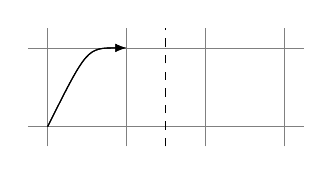
\begin{tikzpicture}
\draw[help lines] (-.25, -.25) grid (3.25, 1.25);
\draw[-latex] (0,0) .. controls (.5,1) .. (1,1);

\draw[dashed] (1.5, -.25) -- (1.5, 1.25);
\pgfexttransformxmirror{1.5}

\draw[-latex] (0,0) .. controls (.5,1) .. (1,1);
\end{tikzpicture}
\end{codeexample}
\end{command}

\switchcolumn% >

\begin{command}{\pgfexttransformxMirror\marg{value}}\cmdcompat\pgftransformxMirror
  Sets up a transformation that mirrors along a vertical line that goes through point $(\text{\meta{value}}, 0)$.

\begin{codeexample}[preamble=\usepgflibrary{ext.transformations.mirror}]
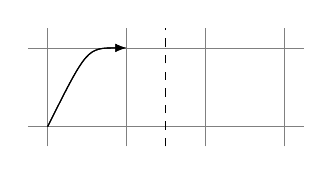
\begin{tikzpicture}
\draw[help lines] (-.25, -.25) grid (3.25, 1.25);
\draw[-latex] (0,0) .. controls (.5,1) .. (1,1);

\draw[dashed] (1.5, -.25) -- (1.5, 1.25);
\pgfexttransformxMirror{1.5}

\draw[-latex] (0,0) .. controls (.5,1) .. (1,1);
\end{tikzpicture}
\end{codeexample}
\end{command}

\switchcolumn*% <

\begin{command}{\pgfexttransformymirror\marg{value}}\cmdcompat\pgftransformymirror
  Sets up a transformation that mirrors along a horizontal line that goes through point $(0, \text{\meta{value})}$.
\end{command}

\begin{command}{\pgfexttransformmirror\marg{point A}\marg{point B}}\cmdcompat\pgftransformmirror
  Sets up a transformation that mirrors along the line that goes through \meta{point A} and \meta{point B}.
 
\begin{codeexample}[preamble=\usepgflibrary{ext.transformations.mirror}]
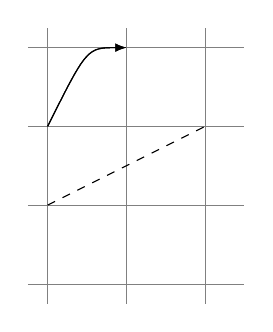
\begin{tikzpicture}
\draw[help lines] (-.25, -2.25) grid (2.5, 1.25);
\draw[-latex] (0,0) .. controls (.5,1) .. (1,1);

\draw[dashed] (0, -1) -- (2, 0);
\pgfexttransformmirror{\pgfpointxy{0}{-1}}
                      {\pgfpointxy{2}{ 0}}

\draw[-latex] (0,0) .. controls (.5,1) .. (1,1);
\end{tikzpicture}
\end{codeexample}
\end{command}

\switchcolumn% >

\begin{command}{\pgfexttransformyMirror\marg{value}}\cmdcompat\pgftransformyMirror
  Sets up a transformation that mirrors along a horizontal line that goes through point $(0, \text{\meta{value})}$.
\end{command}

\begin{command}{\pgfexttransformMirror\marg{point A}\marg{point B}}\cmdcompat\pgftransformMirror
  Sets up a transformation that mirrors along the line that goes through \meta{point A} and \meta{point B}.
 
\begin{codeexample}[preamble=\usepgflibrary{ext.transformations.mirror}]
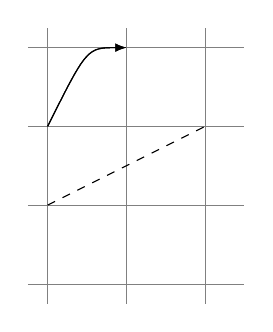
\begin{tikzpicture}
\draw[help lines] (-.25, -2.25) grid (2.5, 1.25);
\draw[-latex] (0,0) .. controls (.5,1) .. (1,1);

\draw[dashed] (0, -1) -- (2, 0);
\pgfexttransformMirror{\pgfpointxy{0}{-1}}
                      {\pgfpointxy{2}{ 0}}

\draw[-latex] (0,0) .. controls (.5,1) .. (1,1);
\end{tikzpicture}
\end{codeexample}
\end{command}

\switchcolumn*% <

\begin{command}{\pgfextqtransformmirror\marg{point A}}\cmdcompat\pgfqtransformmirror
  Sets up a transformation that mirrors along the line that goes through the origin and \meta{point A}.

\begin{codeexample}[preamble=\usepgflibrary{ext.transformations.mirror}]
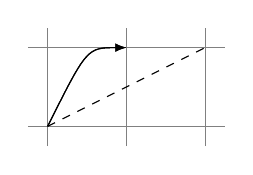
\begin{tikzpicture}
\draw[help lines] (-.25, -.25) grid (2.25, 1.25);
\draw[-latex] (0,0) .. controls (.5,1) .. (1,1);

\draw[dashed] (0, 0) -- (2, 1);
\pgfextqtransformmirror{\pgfpointxy{2}{1}}

\draw[-latex] (0,0) .. controls (.5,1) .. (1,1);
\end{tikzpicture}
\end{codeexample}
\end{command}

\switchcolumn

\begin{command}{\pgfextqtransformMirror\marg{point A}}\cmdcompat\pgfqtransformMirror
  Sets up a transformation that mirrors along the line that goes through the origin and \meta{point A}.

\begin{codeexample}[preamble=\usepgflibrary{ext.transformations.mirror}]
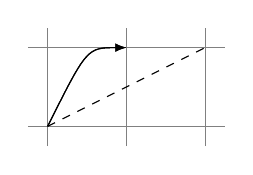
\begin{tikzpicture}
\draw[help lines] (-.25, -.25) grid (2.25, 1.25);
\draw[-latex] (0,0) .. controls (.5,1) .. (1,1);

\draw[dashed] (0, 0) -- (2, 1);
\pgfextqtransformMirror{\pgfpointxy{2}{1}}

\draw[-latex] (0,0) .. controls (.5,1) .. (1,1);
\end{tikzpicture}
\end{codeexample}
\end{command}

\end{paracol}
\endinput


\clearpage
\part{Miscellaneous}

% !TeX spellcheck = en_US
% !TeX root = tikz-ext-manual.tex
% Copyright 2022 by Qrrbrbirlbel
%
% This file may be distributed and/or modified
%
% 1. under the LaTeX Project Public License and/or
% 2. under the GNU Free Documentation License.
%

\begin{tikzlibrary}{misc}
  This library adds miscelleaneos utilities to PGFmath, PGF or \tikzname.
\end{tikzlibrary}

\section{PGFmath}

\subsection{Postfix operator \texttt{R}}

Similar to |\segments[<num>]| in PSTricks, the postfix operator |R| allows the user
to use an arbitrary number of segments of a circle to be used instead of an angle.

\begin{key}{/tikz/full arc=\meta{num} (default |{}|)}
  The number \meta{num} of segments will be set up.
  Using |full arc| with an empty value disables the segmentation and |1R| equals $1^\circ$.
  
  The given value \meta{num} is evaluated when the key is used and doesn't change when
  \meta{num} contains variables that change.
\end{key}
The |R| operator can then be used.
\begin{math-operator}{R}{postfix}{fullarc}
  Multiplies \mvar{x} with $\frac{360}{\meta{num}}$.
\end{math-operator}

\subsection{Functions}

\begin{math-function}{strrepeat("\mvar{Text}", \mvar{x})}
\mathcommand
  Returns a string with \mvar{Text} repeated \mvar{x} times.

\begin{codeexample}[]
\pgfmathparse{strrepeat("foo", 5)} \pgfmathresult
\end{codeexample}
\end{math-function}

\begin{math-function}{isInString("\mvar{String}", "\mvar{Text}")}
\mathcommand
  Returns |1| (true) if \mvar{Text} contains \mvar{String},
  otherwise |0| (false).

\begin{codeexample}[]
\pgfmathparse{isInString("foo", "bar")} \pgfmathresult
\ and\ 
\pgfmathparse{isInString("foo", "foobar")} \pgfmathresult
\end{codeexample}
\end{math-function}

\begin{math-function}{strcat("\mvar{Text A}", "\mvar{Text B}", …)}
\mathcommand
  Returns the concatenation of all given parameters.

\begin{codeexample}[]
\pgfmathparse{strcat("blue!", int(7*3), "!green")} \pgfmathresult
\end{codeexample}
\end{math-function}


\begin{math-function}{isEmpty("\mvar{Text}")}
\mathcommand
  Returns |1| (true) if \mvar{Text} is empty, otherwise |0| (false).
  %
\begin{codeexample}[]
\pgfmathparse{isEmpty("foo")} \pgfmathresult\ and\ 
\pgfmathparse{isEmpty("")}    \pgfmathresult\ and\ 
\def\emptyText{}
\pgfmathparse{isEmpty("\emptyText")} \pgfmathresult
\end{codeexample}
\end{math-function}

\begin{math-function}{atanXY(\mvar{x},\mvar{y})}
\mathcommand
  Arctangent of $\mvar y\div \mvar x$ in degrees. This also takes into account the quadrant.
  This is just a argument-swapped version of |atan2| which makes it easier to use
  the |\p| commands of the |calc| library.
  \index{atan2@\protect\texttt{atan2} math function}%
  \index{Math functions!atan2@\protect\texttt{atan2}}%
  %
\begin{codeexample}[]
\pgfmathparse{atanXY(3,4)} \pgfmathresult
\end{codeexample}
\end{math-function}
\begin{math-function}{atanYX(\mvar{y},\mvar{x})}
\mathcommand
   Arctangent of $y\div x$ in degrees. This also takes into account the quadrant.
\begin{codeexample}[]
\pgfmathparse{atanYX(4,3)} \pgfmathresult
\end{codeexample}
\end{math-function}

\subsection{Functions: using coordinates}
The following functions can only be used with PGF and/or \tikzname.
Since the arguments are usually plain text (and not numbers) one has to wrap
them in |"|.
\begin{math-function}{anglebetween("\mvar{p1}", "\mvar{p2}")}\mathcommand
  Return the angle between the centers of the nodes \mvar{p1} and \mvar{p2}.
\end{math-function}
\begin{math-function}{qanglebetween("\mvar{p}")}\mathcommand
  Return the angle between the origin and the center of the node \mvar{p}.
\end{math-function}
\begin{math-function}{distancebetween("\mvar{p1}", "\mvar{p2}")}\mathcommand
  Return the distance (in pt) between the centers of the nodes \mvar{p1} and \mvar{p2}.
\end{math-function}
\begin{math-function}{qdistancebetween("\mvar{p}")}\mathcommand
  Return the distance (in pt) between the origin and the center of the node \mvar{p}.
\end{math-function}
\begin{codeexample}[width=6cm,preamble=\usetikzlibrary{calc,misc,through}]
\begin{tikzpicture}
\path (0,0) coordinate (A) + (0:4) coordinate (B) +(75:4) coordinate (C);
\draw (A) -- (B) -- (C) -- cycle;
\foreach \cnt in {1,...,4}{
  \pgfmathsetmacro\triA{distancebetween("B","C")}
  \pgfmathsetmacro\triB{distancebetween("C","A")}
  \pgfmathsetmacro\triC{distancebetween("A","B")}
  \path (barycentric cs:A=\triA,B=\triB,C=\triC) coordinate (M)
       node [draw, circle through=($(A)!(M)!(C)$)] (M) {};
  \draw ($(C)-(A)$) coordinate (vecB)
      (M.75-90) coordinate (@)
      (intersection of @--[shift=(vecB)]@ and B--C) coordinate (C) -- 
      (intersection of @--[shift=(vecB)]@ and B--A) coordinate (A);}
\end{tikzpicture}
\end{codeexample}
\section{PGFkeys}

\subsection{Conditionals}

\begin{key}{/utils/if=\meta{cond}\meta{true}\opt{\meta{false}}}
  This key checks the conditional \meta{cond} and applies the styles \meta{true}
  if \meta{cond} is true, otherwise \meta{false}.
  \meta{cond} can be anything that PGFmath understands.
  
  As a side effect on how PGFkeys parses argument, the \meta{false} argument is
  actually optional.
\end{key}

The following keys use \TeX' macros |\if|, |\ifx|, |\ifnum| and |\ifdim| for faster
executions.

\begin{key}{/utils/TeX/if=\meta{token A}\meta{token B}\meta{true}\opt{\meta{false}}}
  This key checks via |\if| if \meta{token A} matches \meta{token B}
  and applies the styles \meta{true} if it does, otherwise \meta{false}.
  
  As a side effect on how PGFkeys parses argument, the \meta{false} argument is
  actually optional.
\end{key}

\begin{key}{/utils/TeX/ifx=\meta{token A}\meta{token B}\meta{true}\opt{\meta{false}}}
  As above.
\end{key}

\begin{key}{/utils/TeX/ifnum=\meta{num cond}\meta{true}\\opt{\meta{false}}}
  This key checks |\ifnum|\meta{num cond}
  and applies the styles \meta{true} if true, otherwise \meta{false}.
  A delimiting |\relax| will be inserted after \meta{num cond}.
  
  As a side effect on how PGFkeys parses argument, the \meta{false} argument is
  actually optional.
\end{key}

\begin{key}{/utils/TeX/ifdim=\meta{dim cond}\meta{true}\opt{\meta{false}}}
  As above.
\end{key}

\begin{key}{/utils/TeX/ifempty=\meta{Text}\meta{true}\opt{\meta{false}}}
  This checks whether \meta{Text} is empty and applies styles \meta{true} if true,
  otherwise \meta{false}.
\end{key}


\subsection{Handlers}

While already a lot of values given to keys are evaluated by PGFmath at some point,
not all of them are.

\begin{handler}{{.pgfmath}|=|\meta{eval}}
  This handler evaluates \meta{eval} before it is handed to the key.
\end{handler}

\begin{handler}{{.pgfmath int}|=|\meta{eval}}
  As above but truncates the result.
\end{handler}

\begin{handler}{{.pgfmath strcat}|=|\meta{eval}}
  As above but uses the |strcat| function.
  
  In the example below, one could have used the |/pgf/foreach/evaluate| key from |\foreach|.
\begin{codeexample}[width=6cm,preamble=\usetikzlibrary{misc}]
\tikz\foreach \i in {0,10,...,100}
  \draw[line width=+.2cm, color/.pgfmath strcat={"red!",sqrt(\i)*10,"!blue"}]
    (0,\i/50) -- +(right:3);
\end{codeexample}
\end{handler}

\begin{handler}{{.List}|=|\meta{\meta{e1}, \meta{e2}, \dots, \meta{en}}}
  This handler evaluates the given list with |\foreach| and concatenates the element and
  the result is then given to the used key.
\begin{codeexample}[width=6cm,preamble=\usetikzlibrary{fit,misc}]
\begin{tikzpicture}[nodes={draw, dashed, inner sep=+10pt}]
  \foreach \point [count=\cnt] in {(0,0), (0,2), (2,0), (2,2), (3,3), (-1,-1)}
    \fill \point circle[radius=.1] coordinate (point-\cnt);
  \node[gray, fit/.List={(point-1),(point-...),(point-4)}] {}; 
  \node[red,  fit/.List={(point-1),(point-...),(point-5)}] {}; 
  \node[blue, fit/.List={(point-1),(point-...),(point-6)}] {};
\end{tikzpicture}
\end{codeexample}
\end{handler}
\begin{center}
\begin{codeexample}[width=10cm,preamble=\usetikzlibrary{graphs,graphdrawing} \usegdlibrary{force}]
\tikzset{
  mynode/.style={
    circle, minimum size=10mm, draw, densely dashdotted, thick,
    decide color/.expand once=#1},
  decide color/.style 2 args={
    /utils/TeX/if=c#1
      {/utils/TeX/ifnum={#2<5}{bluelight}{bluedark}}
      {/utils/TeX/ifnum={#2<8}{light}{dark}}},
  light/.style={fill=gray!20},  bluelight/.style={fill=blue!10},
  dark/.style ={fill=gray!60},  bluedark/.style ={fill=blue!30}}
\tikz\graph[
  spring electrical layout, vertical=c2 to p13,
  node distance=1.5cm, typeset=$n_{\tikzgraphnodetext}$,
  nodes={mynode=\tikzgraphnodetext}] {
  % outer ring
  c2 -- {p1, p11, p6};
    p1 -- {p8, c6, p11};
      p8 -- {p3, p10, c6};
       p3 -- {p13, p15, p10};
         p13 -- {p15, c7};
           c7  -- {c3, c4, p15};
           c3  -- {p14, c4};
           p14 -- {p7, c4};
         p7 -- {p9, p2, c4};
       p9 -- {c5, p12, p2};
     c5 -- {c1, p4, p12};
   c1 -- {p6, p4};
  p6 -- {p11, p4};
  % inner ring
  p11 -- {c6, p12, p4};
  p5 -- {c6 -- {p10, p12}, p10 -- p15, p15 -- c4, c4 -- p2, p2 -- p12, p12 -- p4};
};
\end{codeexample}
\end{center}

\section{PGFfor}

Instead of |\foreach \var in {start, start + delta, ..., end}| one can use
|\foreach \var[use int=start to end step delta]|.

\begin{key}{/pgf/foreach/use int=\meta{start}|to|\meta{end}\opt{|step|\meta{delta}}}
The values \meta{start}, \meta{end} and \meta{delta} are evaluates by PGFmath at initialization.
The part |step |\meta{delta} is optional (\meta{delta} = 1).
\end{key}

\begin{key}{/pgf/foreach/use float=\meta{start}| o|\meta{end}opt{|step|\meta{delta}}}
Same as above, however the results are not truncated.
\end{key}

%TODO: edges to and edges through
\endinput

%%% END
\printindex

%\typeout{Examples: \the\codeexamplecount}%
\end{document}